\section{API}

Neste capítulo, é dado ênfase ao desenvolvimento da API. Como tal, é realizada uma introdução, onde são definidos os requisitos da mesma e são, de maneira reduzida, referidas as tecnologias utilizadas no desenvolvimento desta. De seguida, é apresentada a conceptualização da plataforma e as operações que esta suporta, passando posteriormente para a definição da sua arquitetura e seus sub-módulos. O capítulo é concluído com a realização de uma referência relativamente à base de dados e ao \textit{deployment} da plataforma.

\medskip \par

A \textit{web} API é responsável por estabelecer um serviço RESTful com o qual é possível comunicar sobre HTTPS e que implementa as funcionalidades da plataforma. Esta constitui o \textit{back-end} do projeto e como tal, funciona como fonte de dados para as aplicações cliente.

\medskip \par

Este módulo necessita de cumprir um conjunto de requisitos:

\begin{itemize}
	\item implementar as funcionalidades pretendidas da plataforma, como obtenção de listas de voluntários, registo por parte de utilizadores e outras operações;
	\item interagir com a base de dados;
	\item comunicar sobre HTTPS e suportar autenticação por parte dos clientes.
\end{itemize}

\medskip \par

Tendo em conta o \textit{stack} tecnológico selecionado para desenvolver este projeto, a API foi  desenvolvida em Typescript (sendo que o código é compilado para Javascript) e a mesma é instanciada usando Node.js~\cite{Wilson2018}.

\subsection{Conceptualização}

Tendo em consideração que está a ser desenvolvida uma rede social de voluntariado, foi necessário definir as entidades que estariam disponíveis na plataforma. 

\par \medskip

Relativamente aos utilizadores da plataforma, foram constituídos dois tipos: \textbf{voluntários} e \textbf{organizações}. É necessário haver esta distinção dado que na organização de uma ação de voluntariado estes são dois dos sujeitos participantes mais importantes: aqueles que a organizam (organizações) e aqueles que auxiliam a mesma voluntariamente (voluntários).

\par \medskip

Sendo o propósito da plataforma divulgar este tipo de ações - é necessário definir mais uma entidade: \textbf{eventos}. Estes representam eventos de voluntariado (organizados por organizações registadas na plataforma) que já ocorreram ou que irão ocorrer. É importante também definir que voluntários podem colocar-se como \textit{interessados} num evento - sendo que a partir do momento que estes o façam, é disponibilizado à organização dona do evento o seu contacto.

\par \medskip

Dada a natureza da plataforma é necessário permitir que os utilizadores da plataforma (voluntários e organizações) possam ter uma identidade social de maneira a distinguirem-se dos outros. Sendo assim, foi definido que os utilizadores podem editar o seu perfil (com descrições, contatos e imagens) e realizar \textit{\textbf{posts}}, sendo possível a outros interagir com estes aspetos (na forma de \textit{gostar de posts} e \textit{seguir outro utilizador}).
 
\subsection{Operações}

Levando em consideração o conceito da plataforma definido anteriormente, inicializou-se então a constituição de funcionalidades da API. Definiram-se operações (invocadas através de \textit{endpoints}) que permitem a clientes da plataforma interagir com a mesma, na forma de:

\begin{itemize}
	\item consultar voluntários, organizações, \textit{posts} e eventos;
	\item possibilitar que utilizadores possam criar e editar o seu perfil;
	\item criar \textit{posts} e eventos;
	\item seguir outros utilizadores, gostar de \textit{posts} e ainda marcar o interesse num evento.
\end{itemize}

A referência a todas estas operações encontra-se na \href{https://github.com/leomartins1999/PS1920-G46/wiki}{\textit{wiki}} do projeto.

\subsection{Arquitetura}

A \textit{Web} API, representada na Figura 5, é composta por três módulos: \textbf{controladores}, \textbf{serviços} e \textbf{repositórios} e ainda uma classe principal, responsável por inicializar o servidor e efetuar configurações relacionadas com autenticação e definição de \textit{endpoints}~\cite{Lauret2019,Block2014}.

\begin{figure}[h]
	\centering
	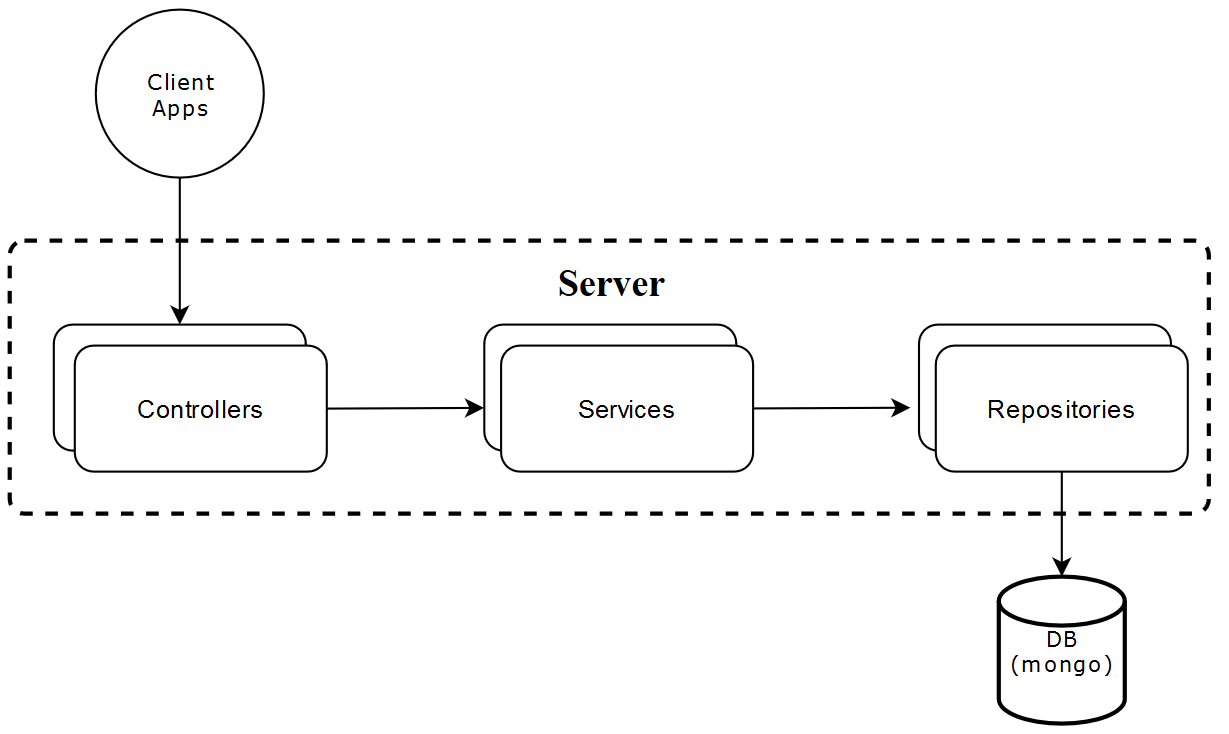
\includegraphics[scale=.30]{api_architeture}
	\caption{Diagrama de arquitetura da API}
\end{figure}

Resumidamente, os \textbf{controladores} têm como responsabilidade a definição de \textit{endpoints} e a realização de chamadas aos serviços, sendo que estes últimos (\textbf{serviços}) tratam a implementação da lógica da aplicação e realização de chamadas aos repositórios. Estes (\textbf{repositórios}) são responsáveis por interagir com à base de dados.

\subsubsection{Controladores}

Tal como já referido, estes definem os \textit{endpoints} existentes na API e invocam o serviço correspondente. No início da execução da aplicação, é instanciado um controlador para cada entidade existente (voluntários, organizações, \textit{posts} e eventos), sendo que nessa instanciação são definidos \textit{endpoints} utilizando o mecanismo de encaminhamento (\textit{routing}) do Express.

\medskip \par

Os controladores tratam também de recolher os parâmetros provenientes nos pedidos HTTPS (contidos no caminho, na \textit{query string}, e no corpo do pedido) e passar os mesmos às funções do serviço, sendo que independentemente do sucesso ou não destas, estes lidam também com a realização das respostas HTTPS.

\subsubsection{Serviços}

Para cada controlador, existe associado a este um serviço. Neste, são definidas as funções que o controlador invoca de maneira a executar a operação pretendida pelo cliente da API.

\medskip \par

Todos os serviços têm uma relação hierárquica de extensão com um serviço base, onde se encontram definidos estaticamente os repositórios de acesso à base de dados. 

\medskip \par

Os serviços, fazendo uso dos repositórios, interagem com a base de dados para implementar a lógica das operações, sendo que o resultado destas é devolvido assincronamente ao controlador.

\subsubsection{Repositórios}

Os repositórios têm como função interagir com a base de dados e devolver o resultado das operações efetuadas assincronamente ao serviço, de maneira a este cumprir a operação solicitada.

\medskip \par

Cada objeto repositório contém uma referência para uma instância de repositório base. Este repositório base é definido genericamente e contém a implementação de operações CRUD sobre a base de dados.

\subsubsection{Autenticação}

De maneira a garantir que os clientes da aplicação possam ter uma experiência personalizada, esta API suporta autenticação através do uso de Passport.js, configurado de maneira a fazer uso de \textit{web cookies}. A partir do momento que um utilizador tem sucesso no processo de autenticação na plataforma, todos os seus pedidos contêm informação relativamente à sessão do mesmo.

\medskip \par

Certas operações na API estão protegidas de maneira a que utilizadores não autenticados não as possam efetuar (como por exemplo a realização de um \textit{post} ou a alteração de um perfil). De maneira a que um utilizador possa aceder a estas, é necessário que este tenha realizado autenticação previamente (e por sua vez, tenha realizado registo na plataforma anteriormente) e que o cliente \textit{web} utilizado por este suporte a utilização de \textit{cookies}.

\subsection{Base de dados}

Tal como introduzido anteriormente, foi tomada a decisão de utilizar MongoDB. MongoDB é um motor de base de dados noSQL, isto é, apresenta um modelo não relacional através da utilização de coleções e documentos.

\medskip \par

Esta escolha implica que todos os documentos numa coleção não necessitam de ter a mesma estrutura, algo que traz alguma flexibilidade e agilidade no processo de desenvolvimento sobre esta plataforma. Outra característica interessante é que os documentos seguem o formato JSON, simplificando a integração destes dados com a aplicação (devido ao uso de Javascript).

\medskip \par

O motor foi selecionado não só para hospedar os dados associados às entidades mas também para albergar o conteúdo das imagens fornecidas pelos utilizadores.

\subsection{Implantação da API}

Tendo em consideração o meio em que o projeto foi desenvolvido, foi tomada a decisão de hospedar a base de dados na máquina onde está implantada (\textit{deployed}) a API (hospedada no serviço Compute Engine da Google Cloud Platform). Contudo, seria mais interessante do ponto de vista de escalabilidade se a mesma fosse hospedada remotamente (através de uma solução \textit{cloud} como o Amazon Web Services ou a Google Cloud Platform) porque possibilitaria a instanciação de múltiplas aplicações API, e consequentemente, a realização de balanceamento de carga.

\medskip \par

A máquina virtual foi configurada com os recursos necessários (como o Node.js) e, numa primeira fase, a aplicação foi instanciada para testes. De maneira a atribuir um nome de domínio ao endereço IP da máquina, foi utilizado o serviço Duck DNS e de seguida, utilizando o CertBot, foi emitido um certificado SSL de maneira a garantir que fosse possível a instanciação da aplicação num modo em que as comunicações fossem realizadas sobre o protocolo HTTPS. A utilização deste protocolo torna a realização de comunicações entre cliente e servidor mais segura devido à encriptação da informação trocada entre ambos. Em plataformas nas quais ocorre a troca de dados sensíveis (como palavras-passe) entre cliente e servidor é essencial a utilização deste protocolo~\cite{Cloudflare2020}.






